\chapter{Research Definition}
\label{chapter-research}

\section{Research Question}\label{research question}

The gaps identified in \cref{chapter-intro} provide the foundation for this masters thesis. The goal will be to develop a framework for and perform a comparative analysis that considers the trade-offs of different methods of decision support. Considerations will include trade-offs in computation, communication to decision makers, similarity of results, and method complexity. Therefore, the research question that will be answered is the following: 

\begin{researchquestion}{Research Question}\label{research-question}
    What are the trade-offs between different methods of decision support when considering a wicked problems and varying policy implementation structures? 
\end{researchquestion}

\section{Approach}
To answer the research question, three identified methods of robust decision support (MORDM, multi-scenario MORDM, and MORO) and their handling of three variations of a wicked policy problem that features tipping point characteristics will be considered. Therefore, a multiple case study approach will be used, which provides a structure for developing a deeper understanding of a theoretical framework or methodology, in this case robust decision support methods, through the analysis of a case or cases of interest \citep{Edwards1998}. The goal of following a structured case study approach and of considering a single case will be to develop generalized conclusions of method trade-offs that can be applied to wicked policy problems with tipping point characteristics \citep{Seawright2008}.

A comparative approach will be incorporated into the case study to ensure rigor in when comparing methods. The comparative method, as defined by \citet{Pennings2006} provides several guidelines to ensure rigor in a comparative analysis. This includes defining the important concepts and points of comparison, establishing the cases that will be used for comparison, and carefully developing causal statements from the established comparisons \citep{Pennings2006}. 

    \subsection{Case Selection}
    Case selection involves seeking a representative sample of cases that include variation along the key dimension under consideration \citep{Seawright2008}. In this case, the key dimension considered is the policy implementation structure of a system. To facilitate method comparison, a highly stylized problem known as the lake problem will be used. This problem features tipping point behavior and is commonly used in existing policy analysis research and bench-marking work. To test the response of each robust decision support method to different policy implementation structures, this stylized problem will be varied to support three levels of policy intervention: a policy with pre-determined and static decisions, a planned adaptive policy that is updated periodically based on a predetermined number of time steps, and a dynamic adaptive policy that is updated after every time step. 

    \subsection{Caveats}
    There are a few recognized pitfalls of using a case study approach to research that must be considered and guarded against. Case studies are often accused of a lack of rigor \citep{Yin2012}, so it will be imperative to monitor the data collection, method application, and results analysis to ensure that rigor is maintained. Second, generalization of results from the selected cases to the wider population can prove problematic \citep{Zainal2007}. Careful selection of the case considered and clear establishment of the research objectives can increase confidence of generalizing the results found \citep{Seawright2008, Yin2012}.

\section{Supporting Questions} \label{def-supporting-questions}
To support the primary research question, several sub-questions will be addressed. This study and, therefore, identified sub-questions, will be structured to follow the commonly accepted IMRAD research framework of Introduction, Methods, Results, And Discussion \citep{Nair2014}. Leveraging such an established framework for research provides structure and helps to ensure that this work is understood and accepted by other researchers.

\begin{enumerate}
    \item \textbf{Introduction}\newline
    Beyond the research definition, this will include establishing a thorough background for the key concepts identified in the research definition
        \begin{itemize}[label={--}]
            \item How is robustness defined in policy analysis? 
            \item What are the origins of the robust decision support methodology?
            \item How have stylized policy problems been leveraged in previous research? 
            \item Does the lake problem incorporate deep uncertainty tipping point behavior? 
            \item What policy implementation structures are commonly recognized in literature?
        \end{itemize}
        
    \item \textbf{Methods}
    Included in this part of the study are the implementation details for each method and problem variation. The framework for comparison is also included in the methodology.  
        \begin{itemize}[label={--}]
            \item What are definitions of the lake problem that represent the three essential types of policy implementation?
            \item How can robustness be determined for each selected robust decision support method?
            \item What are the implementation details for each robust decision support method identified for this study?
            \item What are the points of comparison which should be considered during analysis? 
        \end{itemize}
    
    \item \textbf{Results}
    Results include both an individual analysis of each method and problem variation pairing, as well as a comparison following the framework established in Methods. 
        \begin{itemize}[label={--}]
            \item What are the results from each pairing of robust decision support method and variation of the stylized policy problem?
            \item Based on the points of comparison defined in Methods, how do the results of each pairing compare? 
        \end{itemize}

    \item \textbf{Discussion}
        \begin{itemize}[label={--}]
            \item Based on the points of comparison and definitions of robustness that have been developed, what trade-offs exist between methods and how do methods respond to the different problem variations?
            \item How can the results from this analysis be generalized to other problems and analyses? 
        \end{itemize}
\end{enumerate}

\section{Research Methods}\label{research methods}
Continuing to follow the IMRAD format, this section will discuss methods used for each step in the research process. 

\subsection{Part 1: Introduction}
An extensive review of the literature about each of the robust decision support methods selected will establish the origins and intended implementation of each. Flow charts will be leveraged to identify the specific order of execution for each method. Additional literature review will explore how robustness can defined, both generally in the context of decision making and policy analysis and specifically for individual robustness metrics. The stylized problem and policy structure variations will also be developed from a review of previous applications of the lake problem and research regarding possible policy structures.

\subsection{Part 2: Method}
Development of the identified variations of each stylized policy problem will use Cython, a high performance programming language implemented as a superset of the Python language that allows for the compilation of extremely efficient C code. Using such a high performance language will reduce computing time for these computationally-intensive decision support methods by speeding up the most commonly used process: the problem itself.

This step will also define how each robust decision support method will be executed. The research required to identify proper algorithms for each step of a method will be completed with further literature review of the relevant concepts. Finally, methods will be implemented by leveraging open-source libraries wherever possible to avoid duplicated work and to leverage already well-tested functionality. This will be supplemented with code using Cython when there is potential for a beneficial reduction of processing time. By using Cython for coding needs whenever possible, additional computational power beyond what is available for student use will be minimized as much as possible.

As this research intends to compare multiple methods of robust decision support, it is important to establish how each method is evaluated and how those evaluation methods can be compared. Therefore, literature will be reviewed to determine and quantify points of comparison that will be tracked during execution of each pairing.

\subsection{Part 3: Results}
The results for each method and problem variation will first be determined in isolation, both through data analysis and visual interpretation of results. Visualizations will be built using python-based graphing libraries like Matplotlib and Seaborn. Comparison points established earlier will be then be considered, using mathematical formulas and visualizations where applicable.

\subsection{Part 4: Discussion}
The final step will involve several methods of communication. First, visualizations that summarize the significant results of comparison. Second, the development of a comprehensive thesis that describes the results of each step of research as described in the research definition. All word processing activities will use Latex and relevant templates. The thesis will be submitted to the TU Delft repository and will be made available for download. Finally, code developed for both policy problem variations and for method implementations will be made available through GitHub.

\section{Research Flow}\label{research flow and scheduled}
The research flow found in Figure \ref{fig:flow} provides a guide for the work completed to answer the identified research question. Notice that points of comparison are defined prior to method specification in practice to limit bias when defining metrics, which aims to add validity to the comparison performed in this study. For clarity, however, these metrics will be defined after method and problem development in text.

\begin{figure}[!h]
    \begin{center}
        \captionsetup{width=0.6\textwidth}
        
        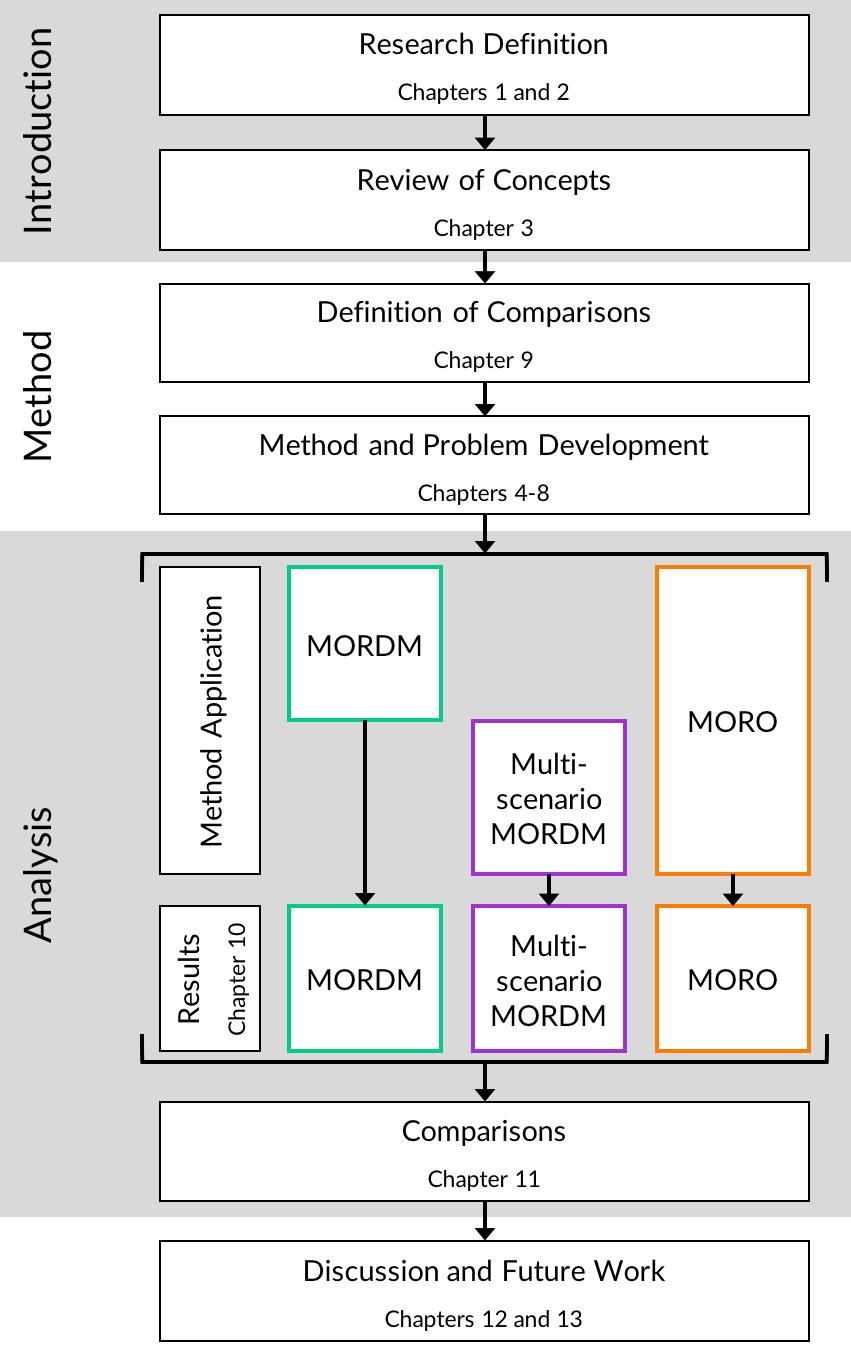
\includegraphics[width=0.6\textwidth]{research-flow}
        \caption{Structure of the work involved this research project}
        \label{fig:flow}
    \end{center}
\end{figure}
